\chapter{Methodology}

\section{Datasets}
\subsection{SEN12-MS}
This thesis relies exclusively on the SEN12MS dataset~\cite{sen12ms_2019}, curated by Schmitt et al.. SEN12MS is a large-scale, globally distributed benchmark explicitly designed to advance research in multimodal Earth observation and deep learning. It comprises 180,662 georeferenced image triplets, each consisting of (i) dual-polarized Sentinel-1 synthetic aperture radar (SAR) data in VV and VH polarization ($\sigma^{0}$ backscatter values in decibel scale), (ii) full Sentinel-2 multispectral imagery spanning all 13 bands, and (iii) MODIS land cover maps derived from the MCD12Q1 product and resampled to 10 m resolution. Each triplet is stored as a 256 × 256 pixel GeoTIFF at 10 m ground sampling distance, corresponding to a spatial coverage of approximately 2.56 × 2.56 km per patch.

The Sentinel-1 component originates from ground-range-detected (GRD) products acquired in interferometric wide swath (IW) mode. These data were radiometrically calibrated and orthorectified against SRTM or ASTER digital elevation models to ensure accurate geolocation. The Sentinel-2 imagery was curated using a cloud-free mosaicking workflow on Google Earth Engine: within each region of interest (ROI), multiple observations collected during a given meteorological season of 2017 were composited such that cloud-contaminated pixels were systematically excluded. This procedure ensured that every ROI is represented by seasonally consistent, nearly cloud-free multispectral data. Finally, the MODIS land cover maps were used to generate categorical reference layers; however, due to their relatively coarse native resolution (500 m), they are subject to spatial inaccuracies even after upsampling.

\begin{figure}[htbp]
    \centering
    % First row: SAR images
    \begin{subfigure}{0.18\textwidth}
        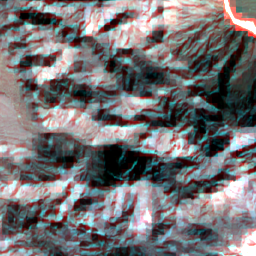
\includegraphics[width=\linewidth]{img/ROIs2017_winter_s2_68_p100.png}
    \end{subfigure}
    \begin{subfigure}{0.18\textwidth}
        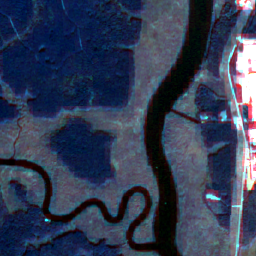
\includegraphics[width=\linewidth]{img/ROIs1970_fall_s2_105_p100.png}
    \end{subfigure}
    \begin{subfigure}{0.18\textwidth}
        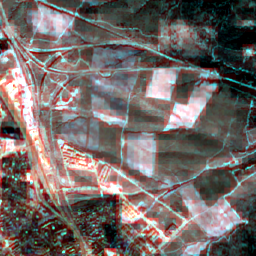
\includegraphics[width=\linewidth]{img/ROIs1970_fall_s2_128_p100.png}
    \end{subfigure}
    \begin{subfigure}{0.18\textwidth}
        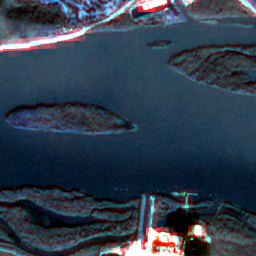
\includegraphics[width=\linewidth]{img/ROIs2017_winter_s2_104_p101.png}
    \end{subfigure}
    \begin{subfigure}{0.18\textwidth}
        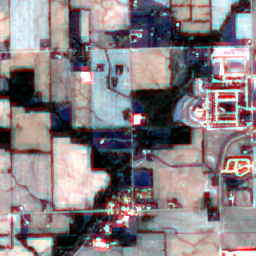
\includegraphics[width=\linewidth]{img/ROIs1970_fall_s2_145_p100.png}
    \end{subfigure}

    \begin{subfigure}{0.18\textwidth}
        \centering
        {\footnotesize \textit{Winter ROI-68-100}}
    \end{subfigure}
    \begin{subfigure}{0.18\textwidth}
        \centering
        {\footnotesize \textit{Fall ROI-105-100}}
    \end{subfigure}
    \begin{subfigure}{0.18\textwidth}
        \centering
        {\footnotesize \textit{Fall ROI-128-100}}
    \end{subfigure}
    \begin{subfigure}{0.18\textwidth}
        \centering
        {\footnotesize \textit{Winter ROI-104-101}}
    \end{subfigure}
    \begin{subfigure}{0.18\textwidth}
        \centering
        {\footnotesize \textit{Fall ROI-145-100}}
    \end{subfigure}
    
    \vspace{0.5em}

    % Second row: MS images
    \begin{subfigure}{0.18\textwidth}
        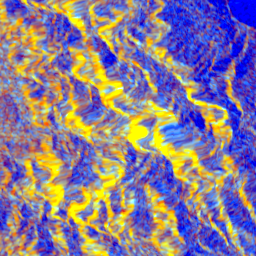
\includegraphics[width=\linewidth]{img/ROIs2017_winter_s1_68_p100.png}
    \end{subfigure}
    \begin{subfigure}{0.18\textwidth}
        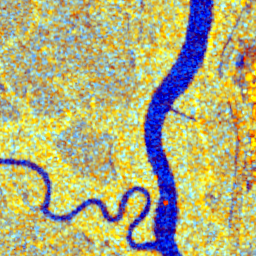
\includegraphics[width=\linewidth]{img/ROIs1970_fall_s1_105_p100.png}
    \end{subfigure}
    \begin{subfigure}{0.18\textwidth}
        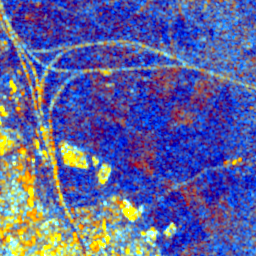
\includegraphics[width=\linewidth]{img/ROIs1970_fall_s1_128_p100.png}
    \end{subfigure}
    \begin{subfigure}{0.18\textwidth}
        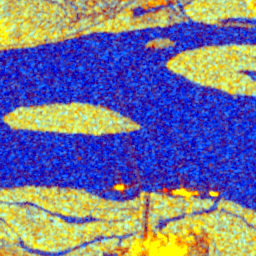
\includegraphics[width=\linewidth]{img/ROIs2017_winter_s1_104_p101.png}
    \end{subfigure}
    \begin{subfigure}{0.18\textwidth}
        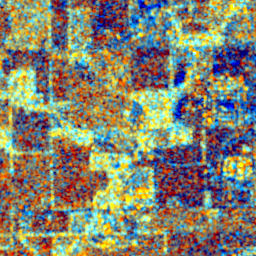
\includegraphics[width=\linewidth]{img/ROIs1970_fall_s1_145_p100.png}
    \end{subfigure}

    \caption{Sample pairs from the SEN12MS dataset. Top row: Sentinel-1 SAR patches (R: VV, G: VH, B: VV/VH). Bottom row: corresponding Sentinel-2 multispectral patches (only RGB bands).}
    \label{fig:sen12ms_pairs}
\end{figure}


Importantly, all triplets underwent manual verification by a remote sensing expert. This revision step ensured that each patch is free from major artifacts, severe registration errors, or residual cloud contamination, thereby guaranteeing the dataset’s quality and usability for machine learning tasks.

The ROIs were sampled globally across all inhabited continents and four meteorological seasons of 2017 to maximize spatial and temporal diversity. Nevertheless, it should be noted that the ROI selection was not purely random. In practice, locations were chosen to avoid large homogeneous areas such as deserts or oceans and to ensure inclusion of diverse land cover classes. While this design improves the dataset’s representativeness for a wide range of applications, it may introduce a bias toward heterogeneous landscapes and thus does not fully capture the true global distribution of land cover types.

For the purpose of this thesis, which addresses translation from SAR to multispectral optical imagery, only the Sentinel-1 and Sentinel-2 modalities are employed. The MODIS land cover products included in SEN12MS are disregarded, as they are not directly relevant to the translation task.

\subsection{SEN12 datasets Family}
SEN12MS is part of a broader line of datasets developed to foster multimodal remote sensing research. Its direct predecessor, SEN1-2~\cite{sen12_2018}, curated by the same research group, contained approximately 282,000 paired patches of Sentinel-1 VV data and Sentinel-2 RGB composites. While groundbreaking in bridging SAR and optical domains, SEN1-2 lacked georeferencing, full spectral coverage, and multi-polarization SAR, limiting its applicability for remote sensing research beyond proof-of-concept image translation.

SEN12MS addressed these limitations by introducing full multispectral coverage, dual-polarized SAR, geocoded products, and auxiliary land cover labels, making it a comprehensive multimodal benchmark. Building upon this foundation, the dataset family has since been extended. SEN12MS-CR~\cite{sen12ms-cr_2021} added temporally matched cloudy and cloud-free Sentinel-2 imagery alongside Sentinel-1 data, enabling the development and benchmarking of cloud removal methods under realistic atmospheric conditions. Subsequently, SEN12MS-CR-TS~\cite{sen12ms-cr-ts_2022} expanded the concept into the temporal domain, providing year-long multimodal time series with 30 co-registered Sentinel-1 and Sentinel-2 acquisitions per ROI. This evolution reflects a progression from simplified SAR–optical pairs, to globally diverse multimodal data, to temporally rich resources designed for time-series analysis and robust cloud removal.

A comparsion of these different datasets is provided in Table~\ref{tab:sen12_datasets}. In this thesis, however, the focus remains on the SEN12MS dataset, leveraging its multimodal SAR and multispectral imagery for the study of SAR-to-optical translation.

% in preamble:
% \usepackage{array,booktabs,adjustbox}
% ragged-right p-columns
\newcolumntype{P}[1]{>{\raggedright\arraybackslash}p{#1}}

\begin{table}[!h]
    \centering
    \caption{Comparison of datasets in the SEN12 family.}
    \label{tab:sen12_datasets}
    \setlength{\tabcolsep}{4pt} % tighter horizontal padding
    \renewcommand{\arraystretch}{1.15} % a bit more vertical room
    \begin{adjustbox}{max width=\textwidth, keepaspectratio=false}
    \begin{tabular}{P{2.6cm} P{3.4cm} P{3.4cm} P{3.6cm} P{3.6cm}}
        \toprule
        \textbf{Aspect} &
        \textbf{SEN1-2}~\cite{sen12_2018} &
        \textbf{SEN12MS}~\cite{sen12ms_2019} &
        \textbf{SEN12MS-CR}~\cite{sen12ms-cr_2021} &
        \textbf{SEN12MS-CR-TS}~\cite{sen12ms-cr-ts_2022} \\
        \midrule
        \textbf{Year released} &
        2018 & 2019 & 2021 & 2022 \\
        \addlinespace[6pt]
        \textbf{Main purpose} &
        Proof-of-concept SAR–optical translation &
        Multimodal learning and data fusion &
        Cloud removal with real cloudy/clear pairs &
        Multi-temporal cloud removal (sequence models) \\
        \addlinespace[6pt]
        \textbf{Modalities} &
        S1 (VV), S2 (RGB) &
        S1 (VV,VH), S2 (13 bands), MODIS LULC &
        S1 (VV,VH), S2 (13 bands; cloudy \& cloud-free) &
        S1 (VV,VH), S2 (13 bands; cloudy \& cloud-free time series) \\
        \addlinespace[6pt]
        \textbf{Georeferencing} &
        Not georeferenced &
        Fully georeferenced &
        Fully georeferenced &
        Fully georeferenced \\
        \addlinespace[6pt]
        \textbf{Spatial sampling} &
        Global patch pairs (282k) &
        180,662 patch triplets across 2017 seasons &
        169 ROIs; $>$100k patch triplets &
        53 ROIs; 30 time steps per ROI \\
        \addlinespace[6pt]
        \textbf{Temporal coverage} &
        Single time-point &
        Seasonal (2017) &
        Seasonal with paired cloudy/clear &
        Year-long time series (2018) \\
        \addlinespace[6pt]
        \textbf{Patch size} &
        $256\times256$ px &
        $256\times256$ px &
        $256\times256$ px &
        $256\times256$ px \\
        \addlinespace[6pt]
        \textbf{Notable limitations} &
        RGB only; VV only; no geocoding &
        MODIS labels are coarse (upsampled) &
        Mono-temporal pairs (no full time series) &
        Fewer ROIs; large storage ($\sim$2\,TB) \\
        \bottomrule
    \end{tabular}
    \end{adjustbox}
\end{table}


\section{Models}

\section{Evaluation Metrics}
